\chapter{Introduction}
\markright{Huijuan Shao \hfill Chapter 1. Introduction \hfill}
Global urbanization has become a trend, and this movement continuously accelerates. 
It has been projected that by the year 2030, cities will grow by 590,000 square miles and add an additional 1.47 billion people, so that 6 out of every 10 people on the planet will live in a city \cite{seto2011meta}. Key issues concerning urban populations; such as public health, sustainable use of limited energy resources, emergency preparedness, and societal stability will rise to the forefront of common discussion. Epidemiological analysis of public health data to analyze infection spread, traffic flow analysis via public transport and taxi cab data, election forecasting and e-governance and the like are just a few of the many examples of how dissecting data about urbanization can provide awareness and knowledge about the society we live in. 

Sustainable energy is a critical issue in this era of urbanization. 
Energy consumption research has long been a topic of research interest, and 
new requirements are continuously being raised in the progress of city development.  
%Towards that end, one of the critical components which has long been a topic of research interest
%but has found resurgence in this era of urbanization is tackling problems of energy consumption.
There is more demand for sustainable energy supply to cities than ever before. The problem of supplying increasing power to cities is two-fold. The immediate impact of urbanization has presented us with logistical problems. How do we meet the needs of the rapidly growing cities? Can we design \emph{smart buildings} and \emph{smart neighborhoods} that optimize energy consumption? Answering these questions is critical to the economy of the country and the economy of the society at large. The larger impact of supplying power to cities is one that the energy industry has on the environment. While renewable energy sources are being investigated, fossil fuels remain the primary source of energy supply. 
  Climate change is a huge problem that will have an impact on humanity as we know it. 
 It is a problem that needs a several-pronged attack to find a solution, and finding solutions to problems in energy consumption, thereby reducing the carbon footprint, would be a big step forward.
 
One of the essential resources in today's world is power and electricity. Needless to say, electricity usage permeates all aspects of modern society.
Its most conspicuous
uses include urban contexts such as
lighting, air conditioning, refrigeration, heating, and powering
appliances and gadgets, but its penetration is pervasive across rural
and industrial sectors.
In 2014, the residential and commercial sector
comprised nearly 40\% of all the electricity generated in the U.S. \cite{book2014us}.
Furthermore, our dependence on electricity will continue to grow
as emphasis shifts away from vehicles that run on fossil fuel to electric
vehicles.

%At another aspect, sensor technology experiences a development from monitoring the power features, to sound and noise, and to the behavior of people by different wireless sensors. 
%Smart buildings is a problem lies in the crossroad of sustainability and controlling. 
Smart building research focuses on the problems associated with energy consumption and maintaining the comfort and satisfaction of people, 
which mainly occurs in inside residential, 
commercial and industrial buildings \cite{hatley2005energy}. 
As shown in Figure \ref{fig_smartbuilding}, 
by using an energy management and control system (EMCS), 
which includes electricity scheduling, 
chilled- and hot-water reset, a thermostat controller, 
and exporting sensor and controller data, 
the buildings can work intelligently to 
achieve the goal of energy efficiency by reducing energy costs, 
maintaining high-level comfort, 
and improving environment friendliness by reducing carbon emissions.
\begin{figure}[h]
\centering
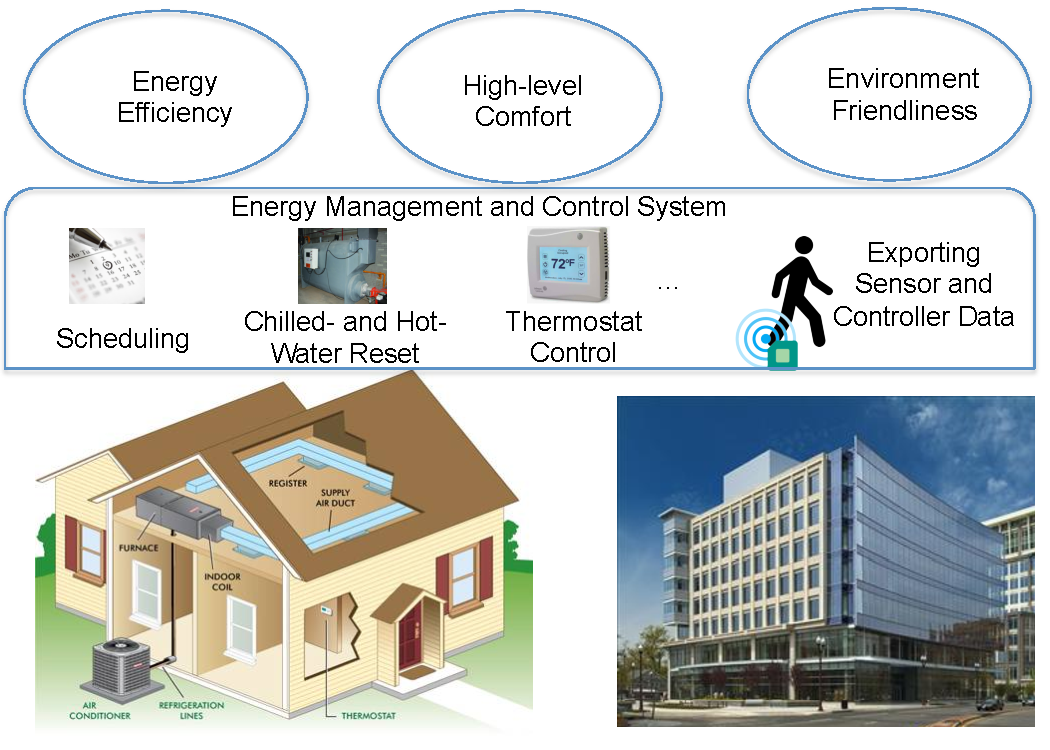
\includegraphics[width=0.8\textwidth]{fig/smartbuilding.pdf}
\caption{Smart Buildings Schema.\label{fig_smartbuilding}}
\end{figure}

%One such application is in \emph{urban computing}, primarily from the perspective of data science. 
%A data scientist role has become critical in being able to learn, process, analyze, and deliver actionable insights that can help realize the promises of this \emph{unprecedented urbanization}. 

\section{Challenges in Smart Building Research}
Smart building aims to achieve significant energy saving by utilizing advanced energy technology. 
The intelligent energy management system monitors devices, controls appliances and conserves energy. To design an energy-saving building, we need to conduct several procedures to achieve this goal. Each change to existing procedures faces different problems. 
\begin{itemize}
  \item Collecting data. 
Determining how to collect accurate energy data using state-of-the-art technology is a fundamental problem. 
  With the advent of sensor technology, wireless sensor nodes and active RFID tags are 
  installed on devices or worn by people to gather comprehensive information \cite{vullers2010energy}. 
Generally, energy consumption, water usage, gas expenditure, air temperature or noise status are monitored by meters or wireless sensors, then the collected data is transmitted to the computer and to storage. 
Identifying how to measure and collect this data precisely with low cost and minimal intrusion has always been a problem. 
  \item Quantify opportunities.
 Analyzing data and discovering opportunities for energy optimization are another concern. 
First we need to identify the devices which consume a large amount of power or water or gas, when they are operated, and the regular patterns of energy consumption. Next, we need to figure out the possible opportunities to decrease energy consumption by evaluating the usage time and energy cost. 
\item Target and Schedule. 
Determining how to set  a reachable target by scheduling the devices inside the building is an optimization subject. When to turn devices on or off, how to set the temperature inside the building without sacrificing the comfort of people, and how to make rules for device automation have been popular research problems. 
\item Track progress.
To evaluate whether a scheduling plan is effective is an important issue. 
How to introduce new technology and update models in time is a challenge. 
%New updated models or technology could be introduced to optimize the energy usage. 
\end{itemize} 

In this dissertation, I focus on quantifying opportunities in energy management. Other issues, such as how to collect energy consumption data, how to schedule the electrical devices or other water use ends, and how to refurbish models to optimize energy usage, are outside the scope of this work. 

%We study two issues in smart buildings research, such as quantify the energy usage of each device with non-intrusive approach (energy disaggregation), occupancy prediction with monitoring sensor of people, which can provide suggestions on the daily plan of heating, ventilation and air conditioning (HVAC) system. 

\section{Goals of this Dissertation}
In this dissertation, I endeavor to clarify the problems of how to qualify energy usage inside buildings. Then I implement existing approaches or enhance current methods to pinpoint energy usage as accurately as possible. This introductory section describes the research motivations, then explains our data-driven models for energy measurement, and concludes with a list of our contributions to smart building research. 

\textbf{Research motivation}

\emph{Analytics} has transformed the perception of the world we live in. Big Data is the lingua franca of the twenty-first century, and data science has become an essential lens through which decision making is seen. The massive amounts of data collected via several active and passive instrumentations positions us truly in an \emph{age of information}. Data via Web 2.0, social media, the internet of things, traffic flow, gene sequencing, etc., in conjunction with the advancement of using data-mining and machine-learning to glean actionable insights, have influenced the world in designing policy, pricing products, launching political campaigns, and many other applications. The power of \emph{data analytics}, thus, is in its diversity. 
With respect to energy quantification, I introduce data-driven models to address several problems that I study in this thesis. 

\textbf{Topic 1: Energy Disaggregation}

While people generally agree on the importance of conservation and
usage curtailment, they often find it difficult to quantify 
{\em where, when} and {\em how much} electricity is consumed.
Typically, residences and businesses receive
monthly electricity bills indicating aggregate usage, with no information on
the breakdown of consumption by appliance/device, time of day, or day of
week (this is an area in great flux, however). Research has 
shown that simply making such feedback available to users
can reduce consumption by up to 50\%, although typical saving 
are in the 9\% to 20\% range \cite{book2014us}.%\cite{energydatabook2011}.

One obvious approach to determining the breakdown of consumption is to install
power meters in every circuit (and sub-circuit)
to capture the consumption of individual devices in homes and
offices. Such installation is costly and intrusive, making 
this option non-viable in practice. 
An alternate
solution, called energy disaggregation or non-intrusive load monitoring
(NILM),
first proposed by Hart~\cite{hart1992}, is using analytics to 
{\em infer} the breakdown of consumption from an aggregate 
power measurement of a
site. This drastically reduces the number of meters required per 
home/installation, typically to just one meter. Furthermore, depending on the analytics desired, it is possible to
use the measurements already being recorded by a utility meter for
disaggregation, especially in cases where utility companies have deployed
smart meters.
Energy disaggregation is hence today a booming area both offering
challenging problems for data analytics and having practical relevance in a
number of areas including sensor networks and building analytics.

\textbf{Topic 2: Disaggregation to Electricity and Water}

Water disaggregation \cite{carboni2016contextualising} is similar to electricity disaggregation. 
By measuring the water flow rate, vibration or pressure in the hot and cold water, 
the flow trace of each water use end is inferred. 
This breakdown process is somewhat different from the electricity disaggregation 
because of the characteristics of water use ends. 

\textbf{Topic 3: Occupancy Prediction}

An effective approach to save energy in homes is to 
efficiently use electric devices.  
In residential buildings, 
the biggest consumer of electricity is the HVAC 
(heating, ventilation, and air conditioning) system, which generally accounts for ~54\% 
of the building's electricity consumption~\cite{book2014us}. 
Determining how to automatically start up and shut down the HVAC unit 
is thus a key problem. 
One solution is to predict the occupancy of a home by analyzing the activities of daily life 
inside the building. 
Based on the occupancy information, 
an automatic control system can then be installed
to operate the HVAC. 

\section{Temporal Data Mining and the Probabilistic Model}
Temporal datasets display a character of time-dependency. 
They are recorded frequently in smart buildings 
and build scenarios to infer the energy usage of people.
 Temporal data mining revolves around the techniques (algorithms) that enumerate structures, patterns, and signatures over temporal data (time series, for instance). 
 A survey \cite{laxman2006survey} has investigated several efficient 
 techniques to discover the patterns in ordered data streams.  
 The techniques used to discover significant patterns vary according to the dataset. 
 One of the compelling patterns in temporal data mining is frequent episodes \cite{mannila1997discovery}.

\textbf{Frequent Episode Discovery}

Frequent episode discovery is proposed in \cite{mannila1997discovery}. 
Given a sequence of events $<(E_1, t_1), ..., (E_n, t_n)>$, 
where $E_i$ denotes the $i^{th}$ event at the time of $t_i$, 
the aim is to find temporal patterns (called \textit{episodes}) that occur 
frequently in the long sequence. 
This episode is an ordered event collections. 
For in-stance an episode $(A\rightarrow B\rightarrow C)$ represents that event type $A$ comes before event type $B$, 
which occurs before event type $C$. 
The occurring time of these events are unnecessary to be consequent. 
The frequency threshold is decided by a user. 
 Several data mining algorithms have been researched to 
 discover the frequent episodes \cite{mannila1997discovery, laxman2005discovering}.
 
\textbf{Motif Mining in Multi-variate Time Series Data}

Motif mining is a temporal data mining technique that was initially proposed in ~\cite{motif1} and \cite{motif2} and extensively studied in \cite{minnen2007improving, tanaka2005discovery, motifgoal}. The fundamental idea behind \emph{motif mining} is that it symbolically encodes the numerical time series data. After this encoding, the symbols combine to form episodes in the data, resulting in patterns that can be mined. Furthermore, by combining domain-specific information and pattern mining techniques, we extract frequent,  meaningful episodes from the symbolized time series.

Furthermore, when there are time series that describe the data, we employ \emph{multi-variate motif mining} to find meaningful patterns. The algorithms for multi-variate temporal motif mining are similar to the univariate case, except that the symbolic encoding is represented as a vector. Therefore each time point in the data is represented as a vector of symbols, with each symbol corresponding to one of the several time series that represents the data. Now, the combination of these vector symbols forms episodes that can be mined from the multi-variate time series data. Again, by combining domain specific knowledge, we extract meaningful episodes from the data.

\textbf{Episode Generating Hidden Markov Model (EGH)} 

A hidden Markov model is a ubiquitous construct to model time series data. It is used to represent probability distributions over a sequence of data. The hidden Markov model gets its name from two important properties. The observation (data point) is generated by a process whose state is \emph{hidden} from the observer. Second, the state of this hidden process satisfies the \emph{Markov} property that the current state is independent of all prior states. The \emph{Episode Generating HMM}, researched in \cite{laxman2005discovering}, connects the episodes with an HMM model and has a parameter to evaluate whether an episode is frequent or not. A mixture of EGH describes a situation in which several frequent episodes are embedded into a time series, and can be used to predict whether a target symbol will be the next symbol in a time series.

\textbf{Applications of Motif Mining and EGH}

In our work we apply motif mining techniques, both univariate and multivariate cases, to energy disaggregation. By correlating episodic information with the switching on and off of appliances from time-series represented energy data, we are able to successfully determine the one-to-one mapping between a certain appliance and its usage patterns and time. 

\begin{figure}[!hbtp]
%\makebox[\textwidth]{\framebox[5cm]{\rule{0pt}{5cm}}}
\centering
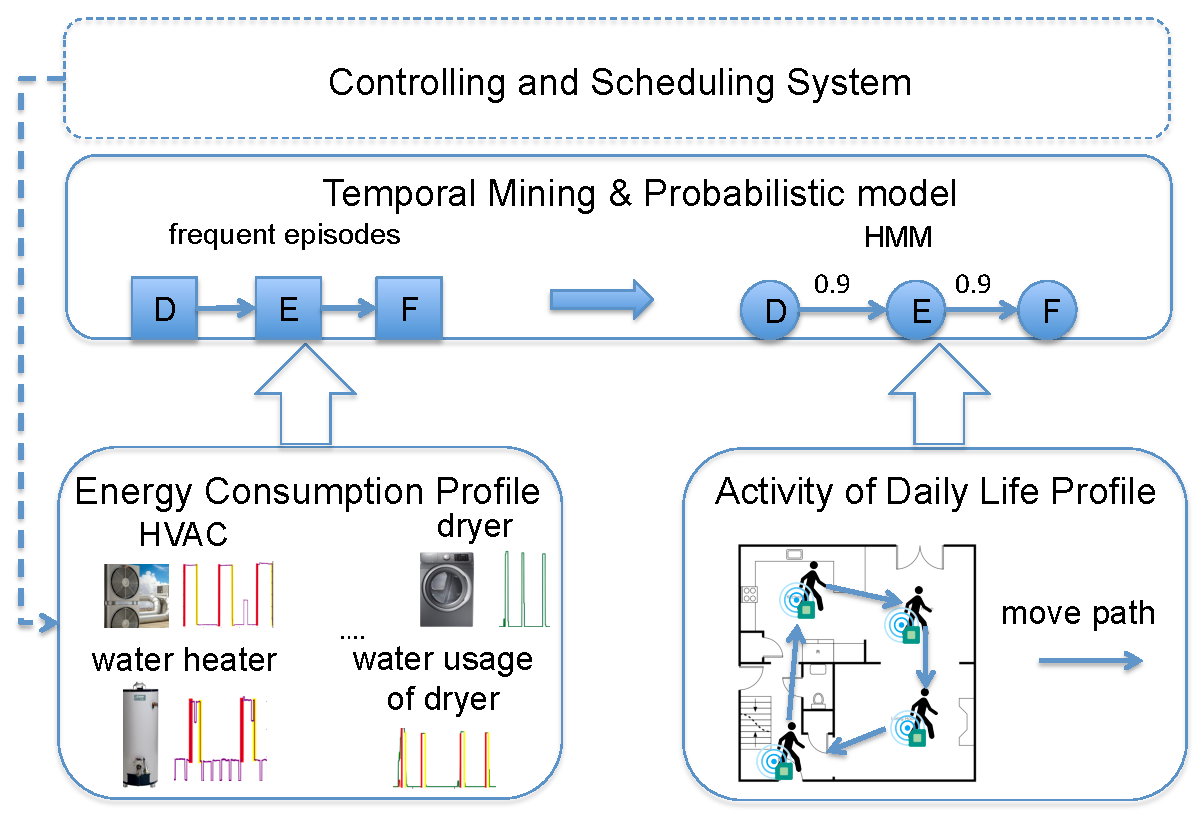
\includegraphics[width=0.7\textwidth]{fig/framework.pdf}
\caption{Overall Framework for Smart Building Issues.\label{fig_framework_whole}}
\end{figure}

Figure \ref{fig_framework_whole} gives a overall framework on the issues of the above smart building issues. 
By mainly collecting the energy consumption of profiles of electrical devices or water use ends, 
and the activities of daily life profiles of people inside buildings, we analyze the frequent episodes from these profiles with temporal mining and probabilistic models. Based on this analysis, a controlling and scheduling system can be developed to control individual devices. 

The formulation of the EGH model lends itself to predicting occupancy in a residence or any building. We develop an EGH model based on occupancy prediction that can assist in automated turning on or off of the HVAC system, which can single-handedly reduce a good portion of the energy consumption footprint. We demonstrate that our algorithm can effectively forecast occupancy.  

\textbf{Contributions}

In this work I make efforts to resolve some of the problems arising in smart building research with 
temporal mining approaches.
\begin{enumerate}
	\item I present a survey on energy disaggregation from the perspective of data mining features and supervised, semi-supervised and unsupervised algorithms. 
	\item The temporal mining approach motif mining works effectively for energy disaggregation. 
	\item I utilize a multivariate piecewise motif mining algorithm for both energy disaggregation and water disaggregation. 
	\item The episode-based model Episode Generating HMM (EGH) and a mixture of EGHs performs well for event prediction in occupancy prediction. 
	%\item It can be used for supervised learning disaggregation and semi-supervised learning approach, even for un-supervised learning approach. 
\end{enumerate}



\section{Organization of this Dissertation}
Smart buildings mainly commit to saving energy in the whole building automatically 
by introducing cutting-edge technologies. The challenges include issues
such as minimizing electricity consumption, decreasing water usage, and automating the heating, ventilation and air conditioning (HVAC) without 
sacrificing comfort. 
In this dissertation, I aim to tackle these issues with data analytics approaches. 
The rest of this report is organized as described below.

\textit{Chapter 2 Survey of Energy Disaggregation:}
In Chapter 2, I survey the energy disaggregation in the past decade from the time it was first proposed, and summarize all the features utilized in the energy disaggregation research. In addition, I categorize the algorithms into classic data mining types. 
I opened the thesis by defining energy disaggregation formally. Briefly, the goal of energy disaggregation is to effectively break down appliance-level power consumption. I then conduct a complete survey of several mechanisms and techniques that employ data mining and machine learning to tackle energy disaggregation. While surveys have been conducted in the past, most of them are presented from an electrical engineering perspective. I survey works that use supervised and unsupervised learning. I compare and contrast a range of algorithms that have been used for energy disaggregation. The self-contained survey used here introduces the electrical engineering concepts that are required for data scientists to conduct research in the space, describe necessary tools and datasets to develop and test algorithms. I describe how experimental testbeds should be setup and how to record data from the necessary sensors and meters. I also present some promising directions for research in energy disaggregation from a data mining perspective. Essentially, we provide a \emph{one-stop-shop} starting point for data mining practitioners to understand the problem scope of energy disaggregation, expose themselves to the problems, and then conduct research in the space.

\textit{Chapter 3 Energy Disaggregation:} In order to curtail electricity consumption, 
we need to capture the usage patterns of the primary electrical devices inside a building. 
In this chapter, I focus on temporal mining algorithms using basic power features to 
separate the dominant electricity consumption devices. I performed experiments on a public 
residential data set and a commercial data set from HP Labs. 

\textit{Chapter 4 Energy and Water Disaggregation:}
In addition to electricity, water is a source of energy spent in buildings.
For the sake of water conservation, 
analyzing water usage patterns in terms of the leading ends of water use is necessary. 
Identifying the major ends of water use is extremely similar to electricity disaggregation. 
This chapter aims to make the temporal mining models applicable to both electricity 
and water disaggregation. 
I conduct an experiment on a dataset which incorporates both electricity and water usage, 
supplied by the University of Virginia. 
The results are presented in Chapter 4.

\textit{Chapter 5 Occupancy Prediction:}
HVAC automation is widely used in commercial and residential buildings. 
Determining how to maximize comfort and minimize electricity usage is a tough issue. 
In this chapter, I target to solve this problem by predicting the occupancy of a room or house. 
I run my temporal mining model as a predictive model to forecast the occupancy status 
of a given day based on the occupancy status of the previous days and the current day. 
I present my analysis in Chapter 5.

\textit{Chapter 6 Conclusion:} This chapter summarizes my work on temporal pattern mining and the associated probabilistic model, and proposes paths for future smart building research. 


%A related problem pertains to
%non-invasive indoor activities tracking.
%The goal here is to predict the locations of people inside a building
%without the use of invasive cameras.

%\section{Timeline}
%The first proposed
%research problem
%on energy disaggregation has been completed although 
%the work will be extended to time-based motif mining and 
%a new probabilistic models.
%The second task of activity of daily life patterns is underway. 
%The third subject on non-invasive indoor activities tracking 
%will start in this Oct.. 
%A timeline of activities is shown in Figure~\ref{fig_PhDtimeline}. 

%\begin{figure}[!hbtp]
%\centering
%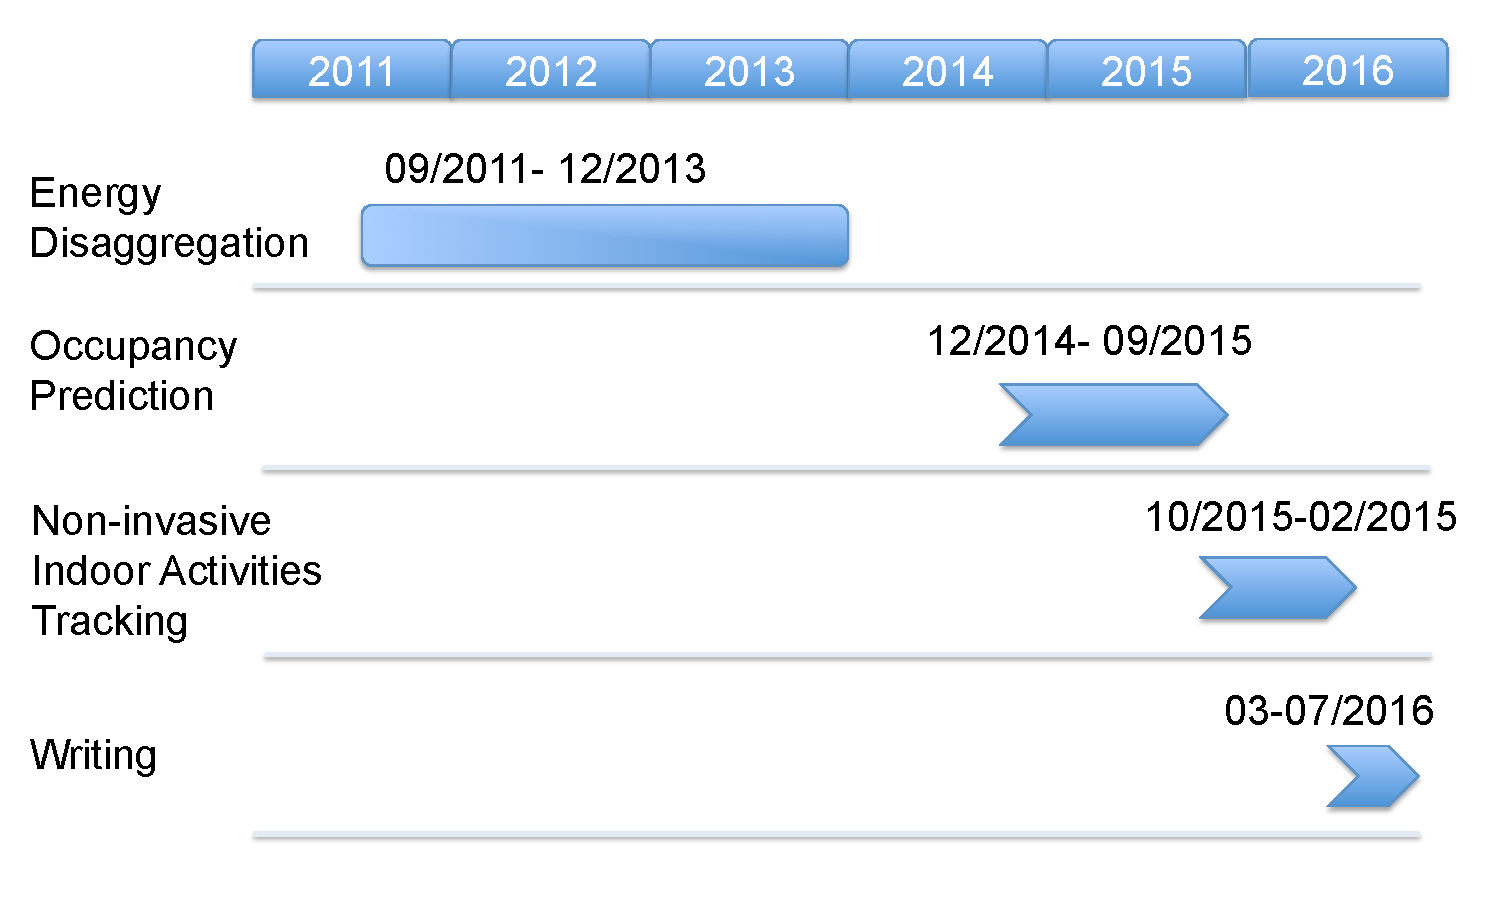
\includegraphics[width=0.8\textwidth]{fig/PhDTimeline.pdf}
%\caption{Timeline.\label{fig_PhDtimeline}}
%x\end{figure}
